\documentclass[journal,12pt,twocolumn]{IEEEtran}
\usepackage{cite}
\usepackage{amsmath,amssymb,amsfonts,amsthm}
\usepackage{algorithmic}
\usepackage{graphicx}
\usepackage{textcomp}
\usepackage{xcolor}
\usepackage{txfonts}
\usepackage{listings}
\usepackage{enumitem}
\usepackage{mathtools}
\usepackage{gensymb}
\usepackage{comment}
\usepackage[breaklinks=true]{hyperref}
\usepackage{tkz-euclide}
\usepackage{listings}
\usepackage{gvv}
\def\inputGnumericTable{}
\usepackage[latin1]{inputenc}
\usepackage{color}
\usepackage{array}
\usepackage{longtable}
\usepackage{calc}
\usepackage{multirow}
\usepackage{hhline}
\usepackage{ifthen}
\usepackage{lscape}
\usepackage{circuitikz}
\usepackage{geometry}

\newtheorem{theorem}{Theorem}[section]
\newtheorem{problem}{Problem}
\newtheorem{proposition}{Proposition}[section]
\newtheorem{lemma}{Lemma}[section]
\newtheorem{corollary}[theorem]{Corollary}
\newtheorem{example}{Example}[section]
\newtheorem{definition}[problem]{Definition}
\newcommand{\BEQA}{\begin{eqnarray}}
\newcommand{\EEQA}{\end{eqnarray}}
\newcommand{\define}{\stackrel{\triangle}{=}}
\theoremstyle{remark}
\newtheorem{rem}{Remark}

\begin{document}

\bibliographystyle{IEEEtran}
\vspace{3cm}

\title{Gate 2022- Instrumentation Engineering}
\author{EE23BTECH11058 - Sindam Ananya$^{*}$% <-this % stops a space
}
\maketitle
\newpage
\bigskip

\renewcommand{\thefigure}{\theenumi}
\renewcommand{\thetable}{\theenumi}

\vspace{3cm}
\textbf{Question 38:} 
Consider the transfer function\\\\
$ H_c(s) = \dfrac{1}{\brak{s+1}\brak{s+3}}$\\\\
Bilinear transformation with a sampling period of $0.1s$ is employed to obtain the discrete-time transfer function $H_d(z)$. Then $H_d(z)$ is 

\begin{enumerate}
\item[(A)] $\frac{(1+z^{-1})^2}{(19-21z^{-1})(23-17z^{-1})}$\\
\item[(B)] $\frac{(1-z^{-1})^2}{(21-19z^{-1})(17-23z^{-1})}$\\
\item[(C)] $\frac{(1+z^{-1})^2}{(21-19z^{-1})(23-17z^{-1})}$\\
\item[(D)] $\frac{(1+z^{-1})^2}{(21-19z^{-1})(17-23z^{-1})}$
\end{enumerate}
\hfill{(GATE IN 2022)}\\
\solution
\begin{table}[h!]
\centering
\begin{tabular}{|c|c|c|}
\hline
\textbf{Parameters} & \textbf{Value} & \textbf{Description}\\
\hline
$ H_c(s) $ & $\dfrac{1}{\brak{s+1}\brak{s+3}}$ & Transfer function in $s$ domain\\
\hline
$T_s$ & $0.1s$ & Sampling period \\
\hline
$H_d(z)$ & & Transfer function of sampled signal\\
\hline
\end{tabular}

\caption{Input Parameters}
\label{tab:gate2022in38table}
\end{table}
\begin{align}
H_c(s) \xleftrightarrow{Bilinear Transform} H_d(z)
\end{align}
To get $H_d(z)$, substitute $s$ with
\begin{align}
s = \frac{2}{T_s}\brak{\frac{1-z^{-1}}{1+z^{-1}}}
\end{align}
where $T_s$ is the sampling period. Then,
\begin{align}
H_d(z) &= \frac{1}{\brak{\frac{2}{0.1}\brak{\frac{1-z^{-1}}{1+z^{-1}}}+1}{\brak{\frac{2}{0.1}\brak{\frac{1-z^{-1}}{1+z^{-1}}}+3}}}\\
&= \frac{(1+z^{-1})^2}{(21-19z^{-1})(23-17z^{-1})}
\end{align}
ROC : $|z| > \frac{19}{21}$\\
Using partial fractions,
\begin{align}
H_d(z) = \frac{1}{323} + \frac{340}{323}\brak{\frac{1}{21-19z^{-1}}} - \frac{380}{323}\brak{\frac{1}{23-17z^{-1}}}
\end{align}
By applying inverse z-transform,
\begin{align}
\delta(n) &\xleftrightarrow{\mathcal{Z}} 1\\
x(0)r^{n}u(n) &\xleftrightarrow{\mathcal{Z}} \frac{x(0)}{1-rz^{-1}}\\
H_d(n) &= \frac{1}{323}\delta(n) + \frac{340}{6783}\brak{\frac{19}{21}}^{n} - \frac{380}{7429}\brak{\frac{17}{23}}^{n}
\end{align}
\begin{figure}[h!]
    \centering
    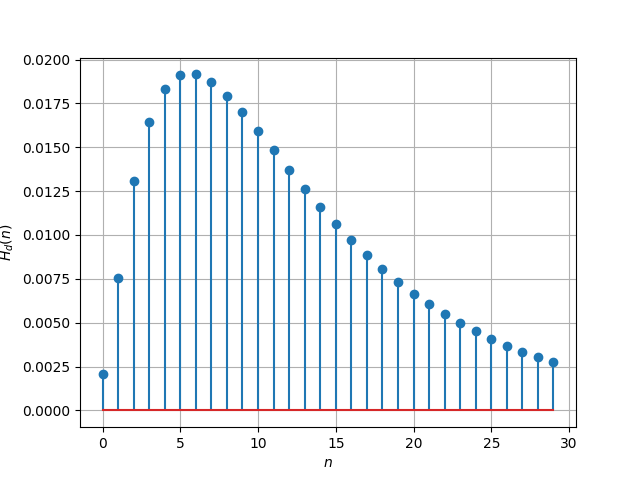
\includegraphics[width=0.8\columnwidth]{figs/plot.png}
    \caption{stem plot of $H_d(n)$}
    \label{fig:gate2022in38fig}
\end{figure}
\end{document}

